% Ubah judul dan label berikut sesuai dengan yang diinginkan.
\section{Checksum}
\label{sec:checksum}

% Ubah paragraf-paragraf pada bagian ini sesuai dengan yang diinginkan.

Sebuah checksum merupakan suatu blok data berukuran kecil yang diperoleh dari blok data digital yang lainnya. Checksum memiliki tujuan untuk mendeteksi error yang mungkin saja terjadi ketika melakukan transmisi data pada memori maupun internet. Checksum biasanya digunakan untuk verifikasi \emph{integrity} dari sebuah data, dengan kata lain apakah datanya sudah dimodifikasi setelah checksum dibuat. Output dari sebuah algoritma fungsi \emph{hash cryptographic}, yang biasa disebut \emph{hashes} atau \emph{digest} digunakan sebagai checksum. Checksum biasanya direpresentasikan dengan menggunakan string hexadecimal (e.g., 69fac420b...), ukurannya berkisar antara 32 sampai 128 digit. Fungsi \emph{hash cryptographic} ini memiliki tiga properti utama, yakni pre-image resistance, second pre-image resistance, dan collision resistance \citep{bart1994}. Fungsi \emph{hash cryptographic} yang sering digunakan adalah MD5, SHA-1, dan SHA-2. MD5 merupakan salah satu fungsi \emph{hash cryptographic} pertama yang dicanangkan. Namun pada akhir 1990an, algoritma tersebut mulai ditinggalkan karena berhasil dirusak sehingga tidak baik untuk keamanan. SHA-1 direkomendasikan oleh National Institute of Standards and Technology (NIST) sampai pada tahun 2015, algoritmanya terbobol. Sekarang, SHA-2 menjadi algoritma terpopuler yang direkomendasikan NIST untuk melakukan verifikasi integritas file \citep{nistpolicy}.

\subsection{MD5}
\label{subsec:MD5}

Sebuah \emph{MD5 message-digest algorithm} adalah hash function yang \emph{cryptographically broken} tapi masih sering digunakan untuk membuat nilai hash 128 bit. \emph{Cryptographically broken} maksudnya adalah secara security sudah tidak aman atau \emph{vulnerable}. Pada awalnya, MD5 didesain sebagai fungsi \emph{hash cryptographic}, namun ditemukan banyak vulnerability pada MD5, yang membuat algoritma ini ditinggalkan. MD5 masih bisa digunakan untuk melakukan verifikasi integritas data, namun hanya untuk mengecek kerusakan data yang tidak disengaja. MD5 masih cocok digunakan untuk hal-hal non kriptografik, seperti menentukan partisi dari kunci tertentu pada database yang sudah dipartisi, dan juga beberapa orang masih memilih menggunakan MD5 daripada \emph{Secure Hash Algorithm} (SHA) karena beban komputasi yang lebih ringan \citep{martin2017}. MD5 didesain oleh Ronald Rivest tahun 1991 untuk menggantikan MD4, dan dispesifikasikan pada tahun 1992 sebagai RFC 1321. Salah satu kebutuhan dasar dari fungsi \emph{hash cryptographic} adalah harus secara komputasional tidak mungkin ditemukan dua buah data yang berbeda dan memiliki nilai hash yang sama. MD5 gagal melakukan hal tersebut dan berdampak cukup fatal. Pada tahun 2019, MD5 tetaplah secara luas digunakan, meskipun kelemahan yang dimiliki sudah banyak didokumentasikan oleh para ahli security \citep{md5vuln}. Sebuah \emph{collision attack} dengan menggunakan komputer 2.6 GHz Pentium 4 dapat menemukan collision pada MD5 dalam hitungan detik. MD5 menggunakan \emph{Merkle–Damgård construction}, jadi jika dua prefix dengan hash yang sama dapat dibuat, maka suffix umum dapat ditambahkan pada keduanya untuk membuat collision yang terjadi dapat diterima dan dianggap valid pada aplikasi yang menggunakannya.

MD5 digest sudah digunakan secara luas pada dunia perangkat lunak untuk memberikan sebuah jaminan dimana file yang ditransmisikan telah tiba dan datanya sama dengan data yang asli. Sebagai contoh, file pada server-server umumnya menyediakan MD5sum yang sudah dikomputasi untuk file tertentu, sehingga user yang mengunduh file tersebut dapat membandingkan apakah file yang diterima sama dan utuh dengan file asli yang terdapat pada server. Kebanyakan UNIX-based system menggunakan MD5sum pada package managernya. ROM pada Android juga menggunakan checksum jenis MD5 ini. MD5 juga biasa digunakan untuk hashing password satu arah, namun NIST tidak merekomendasikan MD5 untuk keperluan ini

\begin{figure} [ht]
  \centering
  % Ubah sesuai dengan nama file gambar dan ukuran yang akan digunakan.
  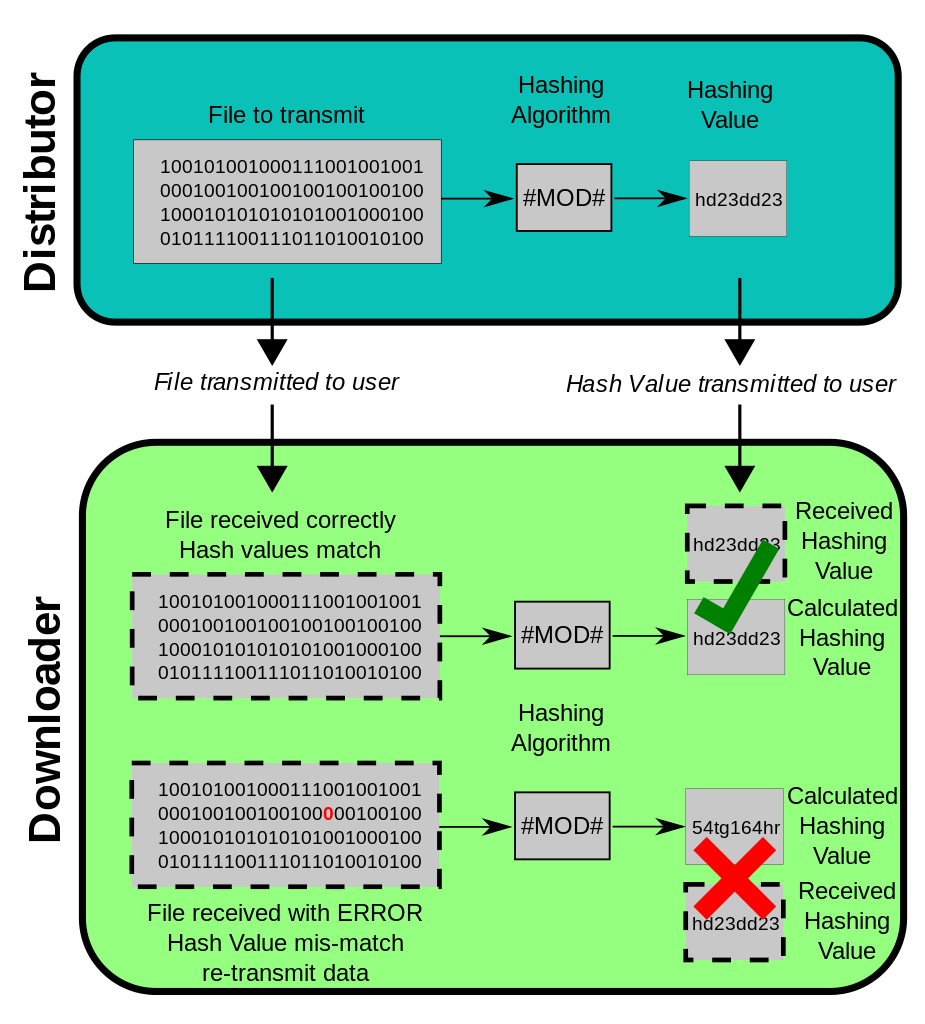
\includegraphics[width=0.4\textwidth]{gambar/hashing-file-transmission.png}

  % Ubah sesuai dengan keterangan gambar yang diinginkan.
  \caption{File transmisi dengan hashing}
  \label{fig:hashingfiletransmission}
\end{figure}

MD5 akan memproses pesan yang memiliki panjang bervariasi menjadi output dengan panjang 128 bit. Pesan masukan dipecah menjadi block-block 512 bit, dan pada pesan dilakukan padding agar panjangnya dapat dibagi dengan 512. Cara paddingnya adalah: pertama, satu bit, 1 ditambah pada akhir pesan. Kemudian bit ini diikuti dengan nol sebanyak yang dibutuhkan untuk membuat panjang message kurang dari 64 bit dari kelipatan 512. Bit sisa yang panjangnya 64 bit diisi dengan 64 bit yang merepresentasikan panjang pesan mulanya, modulo 2.

Algoritma inti dari MD5 bekerja pada keadaan 128-bit, dibagi menjadi 32-bit words, dinotasikan dengan \(A, B, C\), dan \(D\). Variabel tersebut diinisialisasi ke konstanta tertentu. Algoritma inti akan menggunakan tiap blok pesan berukuran 512-bit untuk memodifikasi statenya. Pemrosessan dari blok pesan terdiri dari 4 tahap, termed rounds; tiap tahap terdiri dari 16 operasi yang mirip berdasarkan fungsi linear \(F\), penjumlahan modular, dan rotasi ke kiri. Berikut persamaannya. Terdapat 4 fungsi yang mungkin terjadi, fungsi berbeda digunakan untuk tiap tahapan atau round.

\label{eq:md5sum}
\[ F(B,C,D) = (B \land C) \lor (\neg B \lor D) \]
\[ G(B,C,D) = (B \land D) \lor (B \lor \neg D) \]
\[ H(B,C,D) = B \oplus C \oplus D \]
\[ I(B,C,D) = C \oplus (B \lor \neg D) \]

% Contoh input potongan kode dari file.
\lstinputlisting[
  language=Python,
  caption={Program python sederhana untuk cek md5sum},
  label={lst:md5sum}
]{program/md5sum.py}

Pada Listing \ref{lst:md5sum} adalah contoh program python sederhana untuk melakukan checksum menggunakan MD5. Program tersebut menggunakan library bawaan bernama hashlib.

\subsection{SHA-1}
\label{subsec:SHA1}

SHA-1 merupakan fungsi \emph{hash cryptographic} yang menerima input lalu akan mengeluarkan output 160-bit (20 byte) nilai hash yang dikenal sebagai \emph{message digest}, yang biasanya adalah angka hexadesimal dengan panjang 40 digit. SHA-1 dibuat oleh NSA, badan keamanan Amerika. Sejak tahun 2005, SHA sudah tidak dianggap aman oleh badan-badan keamanan \citep{schneier2005}. NIST secara formal tidak memperbolehkan penggunaan SHA pada tahun 2013. Penggantian SHA-1 terbilang urgent pada penggunaannya dalam digital signature seperti SSL certificate. Semua web browser populer tidak menerima sertifikat SSL SHA-1 pada tahun 2017 \citep{mozilla2019,google2015}. SHA-1 memproduksi message digest dan prinsipnya mirip dengan MD5, namun membuat nilai hash yang lebih besar (160 bit vs 128 bit). Version control system seperti Git, Mercurial, dan Monotone menggunakan SHA-1 bukan untuk sekuriti, namun untuk pengecekan revisi dan untuk menjamin datanya tidak berubah karena korup yang tidak disengaja.

Untuk hash function yang mana \(L\) adalah jumlah bit di message digest, menemukan message yang sesuai dengan message digest dapat selalu dilakukan dengan metode \emph{brute force} yang kira-kira dilakukan \(2^L\) iterasi. Ini dinamakan preimage attack dan mungkin bekerja mungkin juga tidak tergantung dari \(L\) dan kekuatan komputasi dari komputer. Akan tetapi, sebuah \emph{collision}, yang terdiri dari menemukan dua pesan berbeda yang menghasilkan message digest yang sama memerlukan kurang lebih \(1.2\times{2^{L/2}}\) iterasi apabila menggunakan birthday attack. Beberapa aplikasi yang menggunakan cryptographic hashes, seperti penyimpanan password, tidak terlalu terdampak oleh collision attack. Membuat password yang bekerja untuk suatu akun membutuhkan preimage attack, dan juga akses ke hash pada password originalnya. Pada kasus tanda tangan dokumen, attacker tidak dapat langsung memalsukan signature dari dokumen yang sudah ada. Attacker harus membuat sepasang dokumen, satu yang tidak merusak, dan satu untuk merusak, dan membuat pemegang \emph{private key} untuk menandatangani dokumen yang tidak merusak.

\lstinputlisting[
  language=Python,
  caption={Program python sederhana untuk cek sha1sum},
  label={lst:sha1sum}
]{program/sha1.py}

Pada Listing \ref{lst:sha1sum} adalah contoh program python sederhana untuk melakukan checksum menggunakan algoritma SHA-1. Program tersebut menggunakan library bawaan bernama hashlib.

\subsection{SHA-2}
\label{subsec:SHA2}

SHA-2 merupakan perubahan yang cukup signifikan dibandingkan pendahulunya, SHA-1. SHA-2 family terdiri atas enam buah hash function dengan digests (nilai hash) yang bernilai 2254, 256, 384 atau 512 bit: SHA-224, SHA-256, SHA-384, SHA-512, SHA-512/224, SHA-512/256. Hash function pada SHA-2 digunakan secara luas pada sejumlah aplikasi dan protokol sekuriti seperti TLS dan SSL, PGP, SSH, S/MIME dan IPsec. SHA-256 digunakan dalam proses autentikasi package software di OS Debian. SHA-256 dan SHA-512 direncanakan untuk digunakan pada DNSSEC \citep{rfc5702}.

\subsection{SHA-3}
\label{subsec:SHA3}

SHA-3 merupakan member terbaru dari family Secure Hash Algorithm (SHA), yang dirilis oleh NIST pada tahun 2015. Meskipun masih satu family, SHA-3 secara internal berbeda dengan SHA-1 dan SHA-2 yang strukturnya seperti MD5. SHA-3 merupakan subset dari \emph{Keccak} \citep{nist2012}. 

Keccak didasari dari pendekatan baru yang dinamakan sponge construction. Sponge construction didasari dari fungsi random atau fungsi permutasi, dan menerima (atau "menyerap", dalam istilah sponge) input data sebanyak apapun, kemudian mengoutput ("memeras") berapapun jumlah datanya, sambil bertindak sebagai \emph{pseudorandom function}. Pada state absorbing, blok pesan di-XOR menjadi subset dari state, yang kemudian ditransformasikan secara keseluruhan menggunakan fungsi permutasi \(f\). Pada state "squeeze", blok-blok output dibaca dari subset yang sama dari state, berselang-seling dengan fungsi transformasi state \(f\). Ukuran dari bagian pada state yang tertulis dan dibaca dinamakan "rate" (dinotasikan sebagai \(r\)), dan ukuran dari bagian yang tidak tersentuh oleh input/output dinamakan capacity (dinotasikan sebagai \(c\)). Kapasitas ini menentukan tingkat dari sekuritinya. Level maksimum dari sekuritinya adalah separuh dari kapasitasnya. Akgoritma dari \emph{Keccak} adalah sebagai berikut.

Fungsi theta terdiri dari tiga persamaan yang melibatkan operasi XOR sederhana dan bitwise cyclic shift.



\lstinputlisting[
  language=Python,
  caption={Program python sederhana untuk cek sha3sum 512 bit},
  label={lst:sha3sum}
]{program/sha3.py}

\subsection{Lorem Ipsum}
\label{subsec:loremipsum}

\lipsum[11]

% % Contoh pembuatan tabel.
% \begin{table}
%   \caption{Contoh tabel sederhana}
%   \label{tab:tabelsederhana}
%   \centering
%   \begin{tabular}{lll}
%     \toprule
%     Heading1 & Heading2 & Heading3  \\
%     \midrule
%     One      & Two      & Three     \\
%     Four     & Five     & Six       \\
%     \bottomrule
%   \end{tabular}
% \end{table}

% Contoh pembuatan potongan kode.
\begin{lstlisting}[
  language=C++,
  caption={Program halo dunia.},
  label={lst:halodunia}
]
#include <iostream>

int main() {
    std::cout << "Halo Dunia!";
    return 0;
}
\end{lstlisting}

\lipsum[12]

% Contoh pembuatan daftar.
\begin{enumerate}
  \item \lipsum[13][1-4]
  \item \lipsum[13][5-8]
  \item \lipsum[13][9-12]
\end{enumerate}

\lipsum[14-15]
